\documentclass[a4paper,11pt]{article}
\usepackage[margin=2.5cm]{geometry}
\usepackage{graphicx}
\usepackage{float}

\begin{document}

\begin{center}



\includegraphics[width=0.5\textwidth]{Green_University_of_Bangladesh_logo.svg.ipng} 


\textbf{\normalsize{ Green University of Bangladesh}} \\
\textbf{\normalsize{Department of Computer Science and Engineering (CSE)}}\\[1cm]

\textbf{\LARGE{Decentralized E-commerce Platform}}\\[1cm]

\begin{table}[H]
    \centering
    \begin{tabular}{|c|c|} \hline
       \textbf{Name} &  \textbf{ID} \\ \hline
       Md Emon Hossain  & 201902009 \\ \hline
        & \\ \hline
       
    \end{tabular}
   
\end{table} 

\vspace{0.5cm}


 
\textbf{\large Submission Date: 30/05/2023}
\vspace{1cm}

\textbf{\large Course Teacher's Name : Farjana Akter Jui}

\begin{center}
\textbf{Lab Report Status}
\end{center}

\begin{table}[h]
\centering
\begin{tabular}{|p{4cm}|p{6cm}|p{4cm}|} \hline
\textbf{Marks} & \textbf{Date}& \textbf{Signature} \\ \hline  
                &              &                     
                   &              &                     \\ \hline


\end{tabular}
\end{table}

\newpage


\begin{center}


\includegraphics[width=0.5\textwidth]{Green_University_of_Bangladesh_logo.svg.png} 


\textbf{\normalsize{ Green University of Bangladesh}} \\
\textbf{\normalsize{Department of Computer Science and Engineering (CSE)}}\\[1cm]

\textbf{\LARGE{Decentralized E-commerce Platform}}\\[1cm]

\begin{table}[H]
    \centering
    \begin{tabular}{|c|c|} \hline
       \textbf{Name} &  \textbf{ID} \\ \hline
       Md Kamrul Jaman Rabbi & 211902012  \\ \hline
         &  \\ \hline
       
    \end{tabular}
   
\end{table} 

\vspace{0.5cm}


 
\textbf{\large Submission Date: 30/05/2023}
\vspace{1cm}

\textbf{\large Course Teacher's Name : Farjana Akter Jui}

\begin{center}
\textbf{Lab Report Status}
\end{center}

\begin{table}[h]
\centering
\begin{tabular}{|p{4cm}|p{6cm}|p{4cm}|} \hline
\textbf{Marks} & \textbf{Date}& \textbf{Signature} \\ \hline  
                &              &                     
                   &              &                     \\ \hline


\end{tabular}
\end{table}



\end{center}

\newpage

\begin{center}
 \textbf{\Large Title: Decentralized E-commerce Platform DFD Level-0,1,2}   


 \vspace{1cm}
The rise of e-commerce has transformed the way people buy and sell goods and services. As more people turn to online shopping, there is a growing need for e-commerce platforms that are secure, efficient, and decentralized. In response to this need, a Decentralized E-commerce Platform (DECP) has been developed to facilitate e-commerce transactions in a more secure and efficient manner.

The DECP is designed to be a decentralized platform that eliminates the need for intermediaries such as banks and payment processors. It is built on a blockchain technology that allows for secure and transparent transactions between buyers and sellers. With the DECP, buyers and sellers can conduct transactions without having to worry about the risk of fraud, as the platform ensures that all transactions are transparent and verifiable.

This lab report will discuss the design and implementation of the DECP, including the features and benefits of the platform. Additionally, it will provide an analysis of the platform's performance and potential use cases in the e-commerce industry.
\end{center}





    

\vspace{1cm}

\begin{center}
 \textbf{\Large OBJECTIVES/AIM}   


\vspace{0.5cm}
 \begin{enumerate}
    \item To explain the purpose of data-flow diagrams. \\
    \item To describe the meaning of the symbols used in data-flow diagrams    \\
    \item To construct simple data-flow diagrams from a textual description.  \\ 
     \item  To develop a new marketing strategy to increase brand awareness and sales  \\
     \item  To design and implement a new software feature that will improve user experience and reduce customer complaints \\
     \item To conduct a market research study to identify potential new product opportunities and target markets for expansion.\\
     \item To improve customer satisfaction ratings  \\
     \item To reduce production costs\\
     \item To increase employee retention rates \\
     \item To develop a new social media campaign that will increase online engagement and followers  \\
     \item To implement a new inventory management system that will improve accuracy and reduce stock outs \\
     \item To design and launch a new website that will improve user experience and increase conversion rates  \\
     \item  To develop a new safety protocol that will reduce workplace accidents and injuries \\
 \end{enumerate}

\end{center}
\newpage


\begin{center}
    \textbf{\Large PROCEDURE / ANALYSIS / DESIGN }
    \vspace{0.5cm} 
\end{center}

 \section{Data Flow Diagram}
A data flow diagram shows how data moves through an information system graphically. It may show the flow of stored data as well as incoming and outgoing data. The DFD makes no reference to how data moves around the system. It is a well-known visual illustration of how information moves through a system. A

clean and obvious DFD can graphically represent the appropriate quantity of the system need. It demonstrates how information enters and exits the system, what modifies the data, and where information is kept.
DFD and Flowchart differ significantly from one another. The flowchart shows how program modules' control flows. DFDs represent the different levels of data flow in the system. There are no branch or control elements in DFD.
 
 A decentralized e-commerce platform is a platform where buyers and sellers can connect without the need for intermediaries. A platform should have:

\begin{enumerate}
        \item User Registration: The platform should allow users to register themselves as either buyers or sellers. \\
    
    \item User Profile: The platform should allow users to create and edit their profiles with details such as name, contact information, address, and payment details. \\

    \item  Product Catalog: The platform should have a catalog of products that are available for purchase. This catalog should be searchable and filterable.

\item Product Listing: Sellers should be able to create listings for their products. They should be able to add details such as product name, description, images, price, and shipping information
\item Product Management: Sellers should be able to manage their listings. They should be able to edit, delete, or mark their listings as sold.
\item Order Management: The platform should allow buyers to place orders for products. Sellers should be able to view and manage orders, mark orders as shipped, and communicate with buyers regarding the status of their orders.
\item ayment Gateway: The platform should integrate with a payment gateway to facilitate transactions between buyers and sellers.
\item Rating and Reviews: The platform should allow buyers to rate and review products and sellers. This feedback can help other buyers make informed decisions.
\item Messaging System: The platform should have a messaging system that allows buyers and sellers to communicate with each other.
\item Dispute Resolution: The platform should have a system in place to resolve disputes between buyers and sellers.
\item Security: The platform should have robust security measures in place to protect user data, prevent fraud, and ensure secure transactions. 

\item Decentralization: The platform should be truly decentralized, with no single entity controlling the platform or user data.
\end{enumerate}


\section{DFD Level-0,1,2 for decentralized ecomerce system}
\vspace{1cm}

In a Level-0 DFD (Data Flow Diagram), the focus is on providing an overview of the entire decentralized e-commerce system. It shows the major components of the system and their interactions at a high level, without going into detailed processes.
In the Level-1 DFD, the major processes in the system are decomposed into sub-processes:

User Registration and Authentication, Product Listing and Search, Payment Processing, Inventory Management, Review and Rating, User Account Management.

In the Level-2 Code DFD, each sub-function from the Level-1 DFD is further decomposed into more detailed functions or activities, following the same pattern.

\begin{enumerate}
    \item Performance: The platform should be able to handle a high volume of traffic and transactions without significant delays or downtime.
    \item Scalability: The platform should be able to scale up or down based on demand without compromising performance or functionality.
    \item Availability: The platform should be available 24/7 to users without any significant downtime or service interruptions.
    \item Reliability: The platform should be reliable and ensure that transactions are completed successfully and without errors.

    \item Security: The platform should be secure and protect user data and transactions from unauthorized access, fraud, and other security threats.
    \item Privacy: The platform should respect user privacy and ensure that user data is protected and not shared without explicit consent.
    \item Usability: The platform should be user-friendly and easy to navigate, with clear instructions and guidance for users.
    \item Accessibility: The platform should be accessible to users with disabilities and support assistive technologies.
    \item Sustainability: The platform should be environmentally sustainable and minimize its carbon footprint and energy consumption.
\end{enumerate}

\newpage


\begin{center}
    \textbf{\Large IMPLEMENTATION }
\end{center}
   \textbf{Decentralized Network:} 
The first step in implementing a decentralized e-commerce platform is to establish a decentralized network. This can be achieved through the use of blockchain technology, which provides a distributed database that can be used to record and verify transactions. The decentralized network should be able to handle large volumes of transactions, ensure data privacy, and prevent double-spending.

\textbf{User Registration and Authentication:}
Once the decentralized network is established, the platform should allow users to register and authenticate themselves securely. The platform should use a decentralized identity system such as self-sovereign identity (SSI) to ensure the validity of user information. Users should be able to create accounts with their personal information and login credentials. The registration process should include email verification to ensure the validity of the user's email address.

\textbf{Product Management:}
The platform should allow vendors to upload their products for sale, including product descriptions, images, and pricing information. The product information should be stored on the decentralized network to ensure transparency and prevent tampering.

\textbf{Order Management:}
The platform should allow users to place orders for products, and vendors should be able to manage their orders. The platform should use smart contracts to automate the order management process, including payment processing and delivery tracking. The smart contracts should be stored on the decentralized network to ensure transparency and prevent tampering.\\


\textbf{Payment Processing:}
The platform should allow users to make payments using a variety of payment methods, including cryptocurrencies and traditional payment methods. The platform should use a decentralized payment system such as a blockchain-based payment system to ensure security and transparency.


\vspace{1cm}

\textbf{DFD Level-0,1,2}
\vspace{0.5cm}

 
 DFD (Data Flow Diagram) is a graphical representation of how data flows within a system. DFDs are commonly used in software development, system analysis, and process modeling. The purpose of using multiple levels in DFDs is to progressively decompose the system into smaller and more manageable parts, making it easier to understand, analyze, and develop. Each level of DFD provides a different level of detail, starting from an overview of the system (Level-0) and drilling down to the lowest level of processes (Level-2) \\


    \textbf{ Level-0 DFD:} Level-0 DFD provides an overview of the entire system and its major processes. It represents the highest level of abstraction and focuses on the interactions between external entities and the system as a whole. Level-0 DFD consists of bubbles representing processes, labeled with their respective names, and arrows indicating the flow of data between processes, external entities, and data stores. It does not show any internal details of the processes.  \\
   \textbf{Level-1 DFD:}
Level-1 DFD expands on the Level-0 DFD by decomposing the major processes into sub-processes. It provides a more detailed view of the system, breaking down the major processes into smaller, manageable components. Each major process in the Level-0 DFD is further broken down into Level-1 DFDs, which depict the inputs, outputs, and data flows of each sub-process.    \\ 
    \textbf{Level-2 DFD:}
Level-2 DFD provides an even more detailed view of the system by decomposing the Level-1 DFDs into further sub-processes. It continues the hierarchical decomposition of processes until a sufficient level of detail is achieved. Level-2 DFDs can further break down sub-processes from Level-1 DFDs into smaller components, showing more specific data flows and interactions.
    





\newpage



\vspace{0.5cm}


\vspace{1cm}

\begin{center}
    \textbf{\Large TEST RESULT / OUTPUT }
    \vspace{0.5cm}

\textbf{DFD Level-0} 

\vspace{0.5cm}

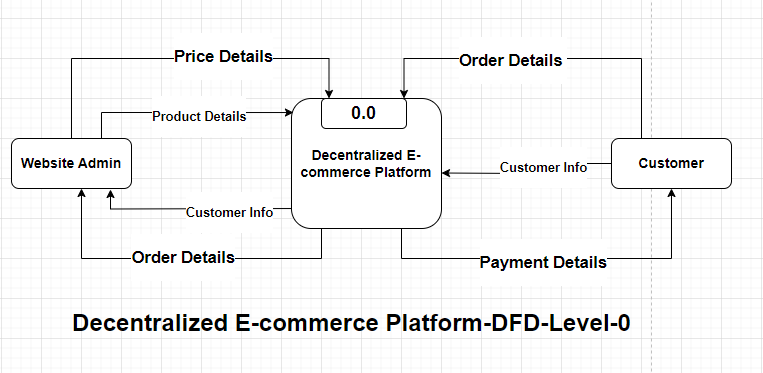
\includegraphics[width=0.5\textwidth]{DFD-Level-0.png} 

\textbf{DFD Level-1}

\vspace{0.5cm}

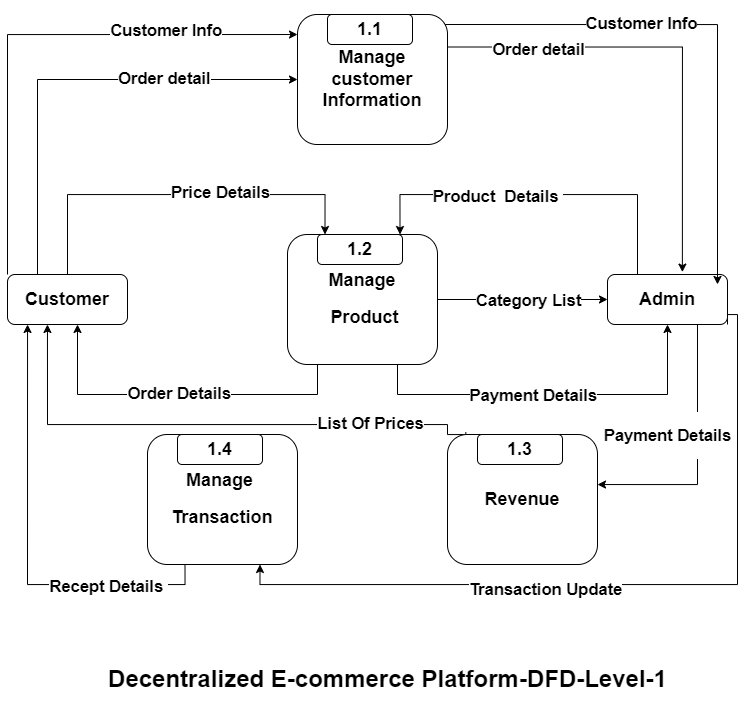
\includegraphics[width=0.5\textwidth]{dfd level-1.png} 

\textbf{DFD Level-2}

\vspace{0.5cm}

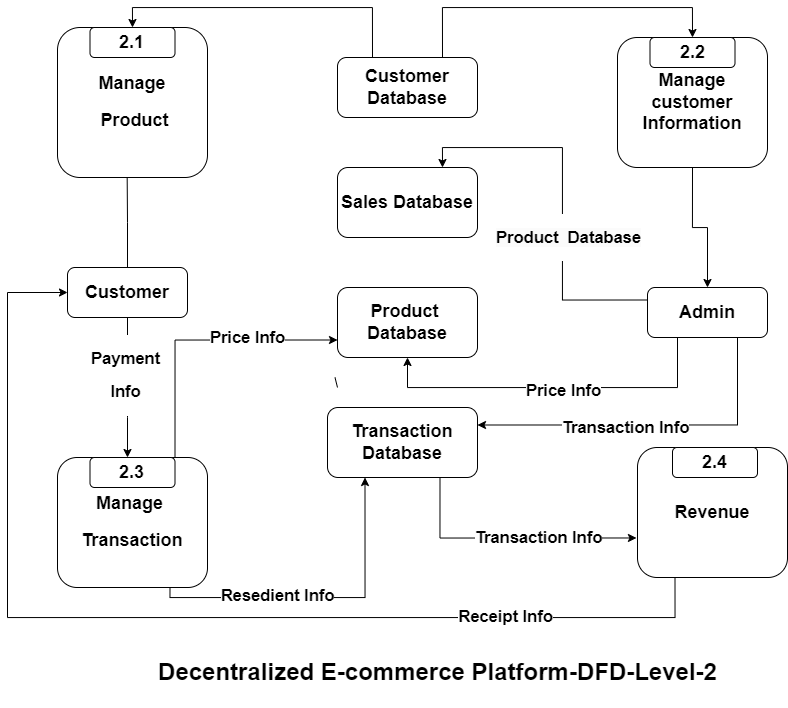
\includegraphics[width=0.5\textwidth]{dfd level-2.png} 

\end{center}



\newpage


\begin{center}
    \textbf{\Large SUMMARY }
    \vspace{1cm}



    
The lab report describes the DFD level-0 , 1, 2 requirements for a decentralized e-commerce platform. The platform aims to provide an alternative to traditional centralized e-commerce platforms, which are often plagued by issues such as high fees, limited control, and privacy concerns.

\vspace{0.5cm}

 DFD Level 0, Gives a high-level overview of the complete decentralized e-commerce system. External entities are users, customers, suppliers, and so on. User Registration and Authentication, Product Listing and Search, Order Placement, Payment Processing, Inventory Management, Review and Rating, and User Account Management are examples of processes.
 \\
Data stores are system-wide storage sites for data.
DFD Level 1, Gives a more in-depth look at the system.
Each significant process at Level-0 is subdivided into Level-1 DFDs. User Registration and Authentication, Product Management, Order Management, Payment Processing, Inventory Management, Review and Rating, and User Account Management are all sub-processes.
\\
 
DFD Level 2, Decomposes Level-1 sub-processes into more particular functions or activities to provide additional detail.
For a more complete understanding, the hierarchical decomposition is continued.

 
\vspace{0.5cm}
Overall, the DFDs help illustrate the flow of data and control within the decentralized e-commerce system, showing interactions between external entities, processes, and data stores. The hierarchy of DFD levels progressively breaks down the system into smaller, more manageable components, allowing for better understanding, analysis, and development of the system.

\vspace{1cm}

\begin{thebibliography}{5}

\vspace{1cm}

\bibitem{kauffman2008}
Kauffman, B. (2008).
``Decentralism."
In R. Hamowy (Ed.),
\textit{The Encyclopedia of Libertarianism}.
Thousand Oaks, CA: Sage, Cato Institute.

\bibitem{deleon1994}
De Leon, D. (1994).
\textit{Leaders from the 1960s: A Biographical Sourcebook of American Activism}.
Greenwood Publishing Group.

\bibitem{roberts1984}
Roberts, N. L. (1984).
\textit{Dorothy Day and the Catholic worker}.
National security essay series, State University of New York Press.

\bibitem{walker2011}
Walker, J. (2011).
``Mark O. Hatfield, RIP."
\textit{Reason}, August 8.

\bibitem{loomis2005}
Loomis, M. J. (2005).
\textit{Decentralism: Where It Came From – Where Is It Going?}.
Black Rose Books.

\end{thebibliography}


   
\end{center}




\end{document}

